\documentclass{beamer}

\usepackage[utf8]{inputenc}
\usetheme{Copenhagen}
\usepackage{amssymb}
\usepackage{pifont}
\usepackage{tikz}
\usetikzlibrary{automata, positioning, arrows}
\usepackage{multirow}



\tikzset{
	state/.style={
		rectangle,
		%   rounded corners,
		draw=black, very thick,
		minimum height=2em,
		inner sep=2pt,
		text centered,
	},
}


\newcommand{\xmark}{\ding{55}}%
\newcommand{\cmark}{\ding{51}}


\title[LTL Motion Planning]{LTL Motion Planning}
\author{F. Barbosa, K. Grover, J. K\v{r}et\'{i}nsk\'{y}, J. Tumova}
%\author{Presented by Kush}
\date{}
\begin{document}
	\frame{\titlepage}
	
	\begin{frame}
		\centering
		\hspace{10pt}
		\begin{figure}
	\centering
    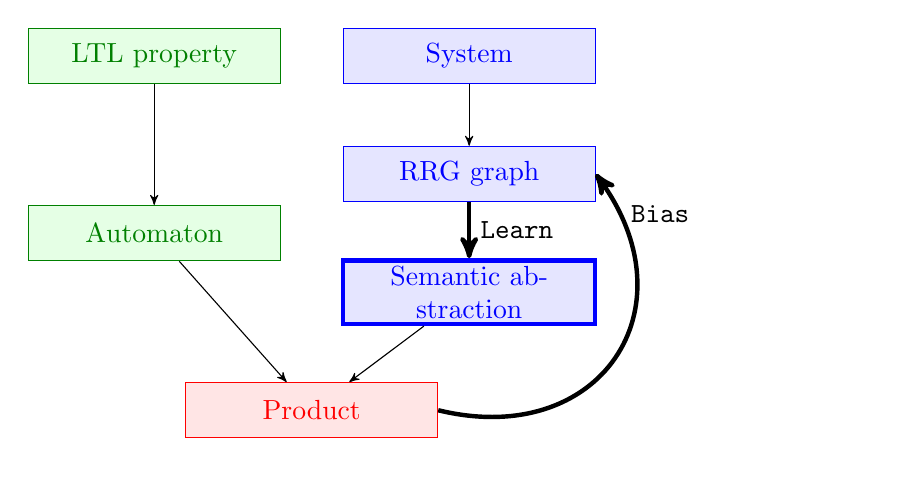
\begin{tikzpicture}[->,>=stealth', minimum width = 32mm,text width = 30mm]
        \node[state=initial, color = blue, anchor=center, fill = blue!10!white,thin] (A) {System};
        \node[state, color = blue, below of = A, fill = blue!10!white, node distance =1.5cm,thin] (B) {RRG graph};
        \node[state, color = blue, below of = B, fill = blue!10!white, node distance =1.5cm,ultra thick] (C) {Semantic abstraction};
        \node[state, color = red, below of = C, fill = red!10!white, xshift = -2cm, node distance =1.5cm,thin] (D) {Product};
        \node[state, color = green!50!black, left of = A, fill = green!10!white, node distance =4cm,thin] (E) {LTL property};
        \node[state, color = green!50!black, below of = E, fill = green!10!white, node distance =2.25cm,thin] (F) {Automaton};
        
        \path (A) edge[] (B)
        (B) edge[ultra thick] node[right,pos=0.5]{\texttt{Learn}} (C)
        (C) edge (D)
        (E) edge (F)
        (F) edge (D)
        (D.east) edge[bend right=70,looseness=1.5, ultra thick] node[right,pos=0.9]{\texttt{Bias}} (B.east)
        %guidance $\rightarrow$ better paths and learning w.r.t. property
        ;
    \end{tikzpicture}
    \caption{Scheme of our model-checking-inspired approach with novel elements drawn thickly. }
    \label{fig:guide}
\end{figure}
	\end{frame}

	\begin{frame}
		\frametitle{LTL Motion Planning}
		\begin{center}
			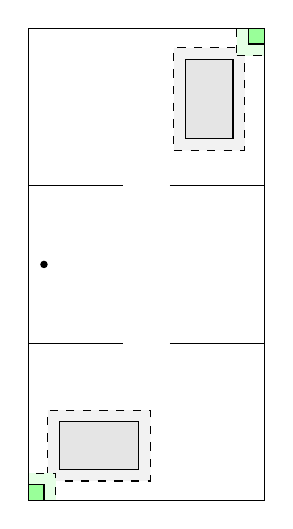
\begin{tikzpicture}
			\filldraw[dashed, fill = gray!10!white] (0.25,0.25) -- (1.55,0.25) -- (1.55,1.15) -- (0.25,1.15) -- (0.25, 0.25);
			\filldraw[dashed, fill = green!10!white] (0,0) -- (0.35,0) -- (0.35,0.35) -- (0,0.35) -- (0,0);
			\filldraw[dashed, fill = gray!10!white] (1.85,4.45) -- (2.75,4.45) -- (2.75,5.75) -- (1.85,5.75) -- (1.85, 4.45);
			\filldraw[dashed, fill = green!10!white] (2.65,5.65) -- (3,5.65) -- (3,6) -- (2.65,6) -- (2.65,5.65);
			
			\filldraw[fill = green!40!white, draw = black] (0, 0) rectangle (0.2, 0.2);
			\filldraw[fill = black!10!white, draw = black] (0.4, 0.4) rectangle (1.4, 1);
			\filldraw[fill = green!40!white, draw = black] (2.8, 5.8) rectangle (3, 6);
			\filldraw[fill = black!10!white, draw = black] (2, 4.6) rectangle (2.6, 5.6);
			
			\draw (0, 0) -- (3, 0) -- (3, 6) -- (0, 6) -- (0, 0);
			\draw (0, 2) -- (1.2, 2) (1.8, 2) -- (3, 2);
			\draw (0, 4) -- (1.2, 4) (1.8, 4) -- (3, 4);
			\filldraw[black] (0.2, 3) circle (0.4mm);
			\end{tikzpicture}
			
			\emph{Specification:} $G F (r_1 \wedge b) \wedge G F (r_2 \wedge b)$
		\end{center}
	\end{frame}


	\begin{frame}
		\frametitle{Building the product}
		\begin{center}
			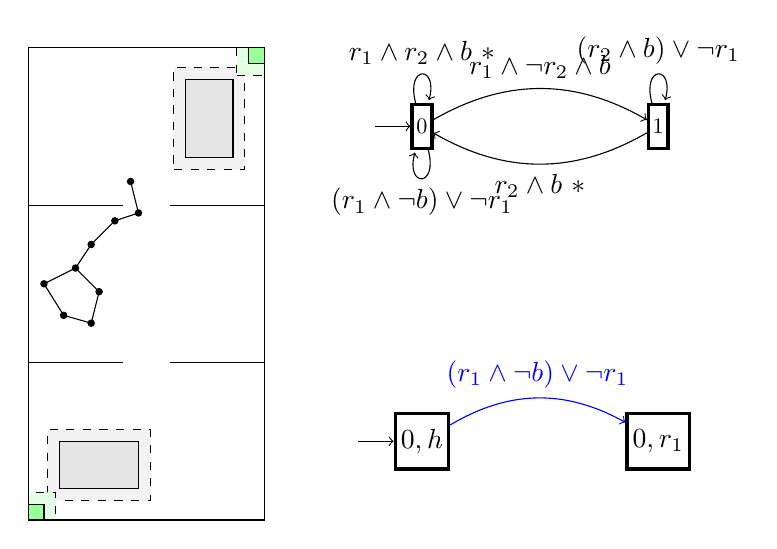
\begin{tikzpicture}
			\filldraw[dashed, fill = gray!10!white] (0.25,0.25) -- (1.55,0.25) -- (1.55,1.15) -- (0.25,1.15) -- (0.25, 0.25);
			\filldraw[dashed, fill = green!10!white] (0,0) -- (0.35,0) -- (0.35,0.35) -- (0,0.35) -- (0,0);
			\filldraw[dashed, fill = gray!10!white] (1.85,4.45) -- (2.75,4.45) -- (2.75,5.75) -- (1.85,5.75) -- (1.85, 4.45);
			\filldraw[dashed, fill = green!10!white] (2.65,5.65) -- (3,5.65) -- (3,6) -- (2.65,6) -- (2.65,5.65);
			
			\filldraw[fill = green!40!white, draw = black] (0, 0) rectangle (0.2, 0.2);
			\filldraw[fill = black!10!white, draw = black] (0.4, 0.4) rectangle (1.4, 1);
			\filldraw[fill = green!40!white, draw = black] (2.8, 5.8) rectangle (3, 6);
			\filldraw[fill = black!10!white, draw = black] (2, 4.6) rectangle (2.6, 5.6);
			
			\draw (0, 0) -- (3, 0) -- (3, 6) -- (0, 6) -- (0, 0);
			\draw (0, 2) -- (1.2, 2) (1.8, 2) -- (3, 2);
			\draw (0, 4) -- (1.2, 4) (1.8, 4) -- (3, 4);
			\filldraw[black] (0.2, 3) circle (0.4mm);
			
			\onslide<2->{
				\node[state,initial,initial text=,scale=0.8] (q1) at (5,5) {$0$};
				\node[state,scale=0.8] (q2) at (8,5) {$1$};
				
				\draw (q1) edge[loop above] node{$r_1 \wedge r_2 \wedge b\ \ast$} (q1);
				\draw (q1) edge[loop below] node{$(r_1 \wedge \neg b) \vee \neg r_1$} (q1);
				\draw (q1) edge[bend left, above, ->] node{$r_1 \wedge \neg r_2 \wedge b$} (q2);
				\draw (q2) edge[loop above] node{$(r_2 \wedge b) \vee \neg r_1$} (q2);
				\draw (q2) edge[bend left, below, ->] node{$r_2 \wedge b\ \ast$} (q1);
			}
		
			\onslide<2->{
				\filldraw[black] (0.6, 3.2) circle (0.4mm);
				\draw (0.2,3) -- (0.6, 3.2);
				\filldraw[black] (0.45, 2.6) circle (0.4mm);
				\draw (0.2,3) -- (0.45, 2.6);
				\filldraw[black] (0.8, 3.5) circle (0.4mm);
				\draw (0.6,3.2) -- (0.8, 3.5);
				\filldraw[black] (0.9, 2.9) circle (0.4mm);
				\draw (0.6,3.2) -- (0.9, 2.9);
				\filldraw[black] (0.8, 2.5) circle (0.4mm);
				\draw (0.45, 2.6) -- (0.8, 2.5);
				\draw (0.9, 2.9) -- (0.8, 2.5);
				\filldraw[black] (1.1, 3.8) circle (0.4mm);
				\draw (0.8, 3.5) -- (1.1, 3.8);
				\filldraw[black] (1.4, 3.9) circle (0.4mm);
				\draw (1.1, 3.8) -- (1.4, 3.9);
				\node[state,initial,initial text=] (0h) at (5,1) {$0,h$};
			}
			
			\onslide<3->{
				\filldraw[black] (1.3, 4.3) circle (0.4mm);
				\draw (1.4, 3.9) -- (1.3, 4.3);
				
				
			}
			\onslide<4->{
				\node[state] (0r1) at (8,1) {$0,r_1$};
				\draw (0h) edge[color = blue, bend left, above, ->] node{$(r_1 \wedge \neg b) \vee \neg r_1$} (0r1);
			}
			
			\end{tikzpicture}
			\onslide<5->{
				\\
				Add transitions ``similar" to this also.
			}
		\end{center}
	\end{frame}


\begin{frame}
	\frametitle{Algorithm}
	\begin{itemize}
		\item Store map of sensing radius. \pause
		\item Sample a batch. \pause
		\item Get bias.\pause
		\item Add frontiers using bias. \pause
		\item Learn from new samples.\pause
		\item Select the best frontier and move.
	\end{itemize}
	
\end{frame}

	\begin{frame}
		\frametitle{Results}
		\centering
		Average taken over 10 runs.
		\begin{table}
			\centering
			\tiny
			\begin{tabular}{|c|c|c|c|c|c|}
				\hline
				\textbf{Environment} & \textbf{Bias} & \textbf{Time taken [s]} & \textbf{RRG size} & \textbf{Movement Length} & \textbf{Remaining length}\\
				\hline
				\multirow{2}{*}{Separate} 
				& No  & 7.54 & 2301 & 60.1 & ? \\
				& Yes & 4.54 & 1171 & 60.1 & ? \\
				\hline
				\multirow{2}{*}{Together} 
				& No  & 10.84 & 3221 & 39.31 & ? (0.8) \\
				& Yes & 8.06  & 2131 & 49.85 & ? (4.3) \\
				\hline
			\end{tabular}
			\caption{Comparison}. \label{tab:results}
		\end{table}
	\end{frame}

\begin{frame}
	\frametitle{A run}
	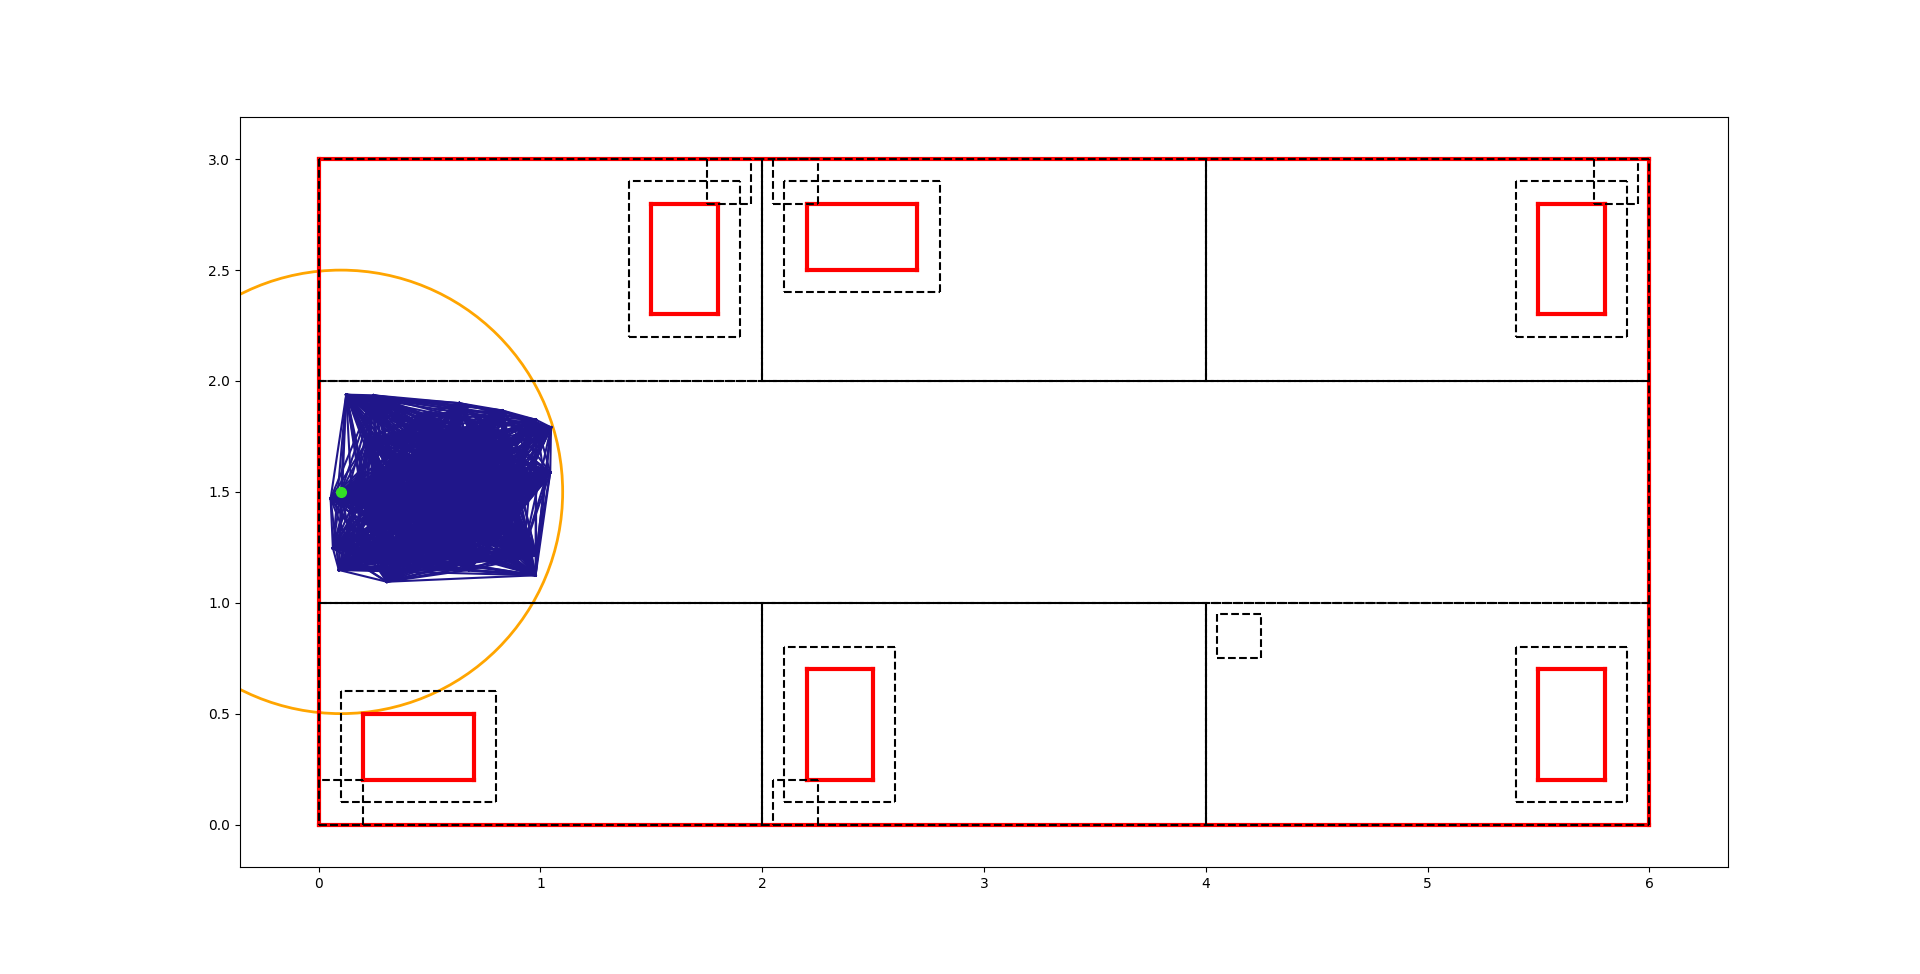
\includegraphics[width=\textwidth]{firstMove.png}	
\end{frame}

\begin{frame}
	\frametitle{A run}
	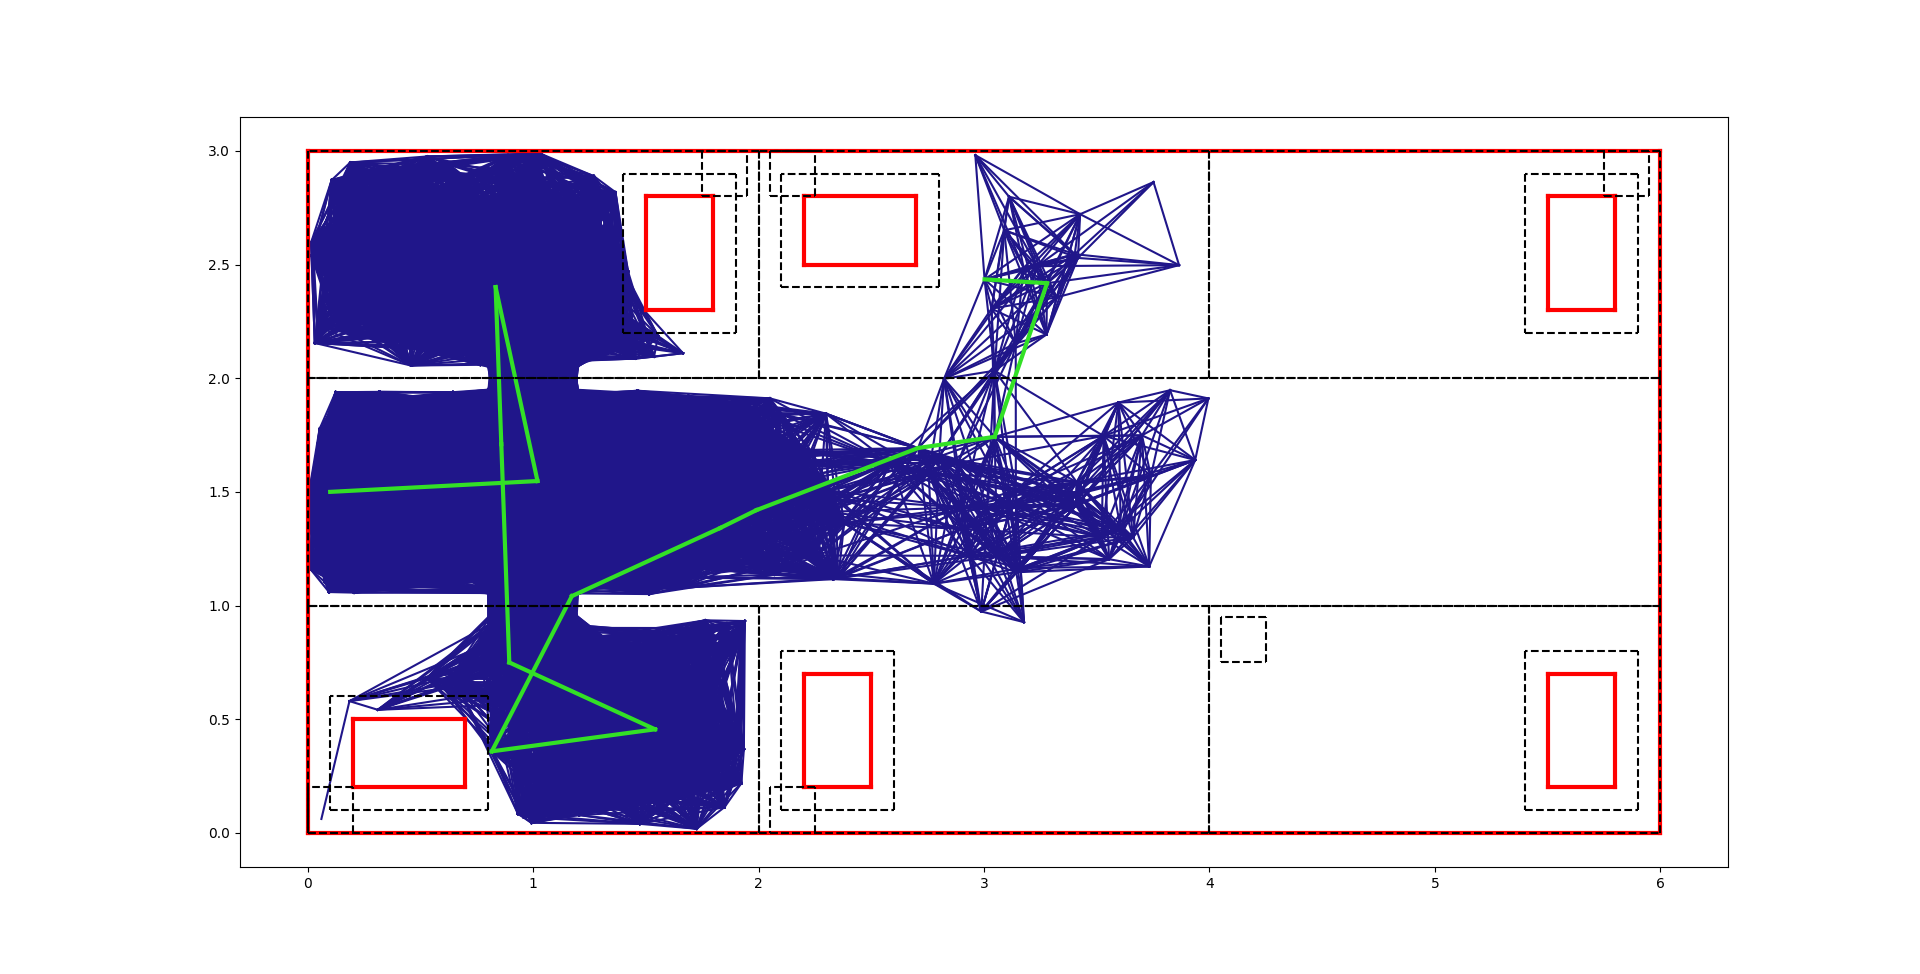
\includegraphics[width=\textwidth]{bin.png}
\end{frame}

\begin{frame}
	\frametitle{A run}
	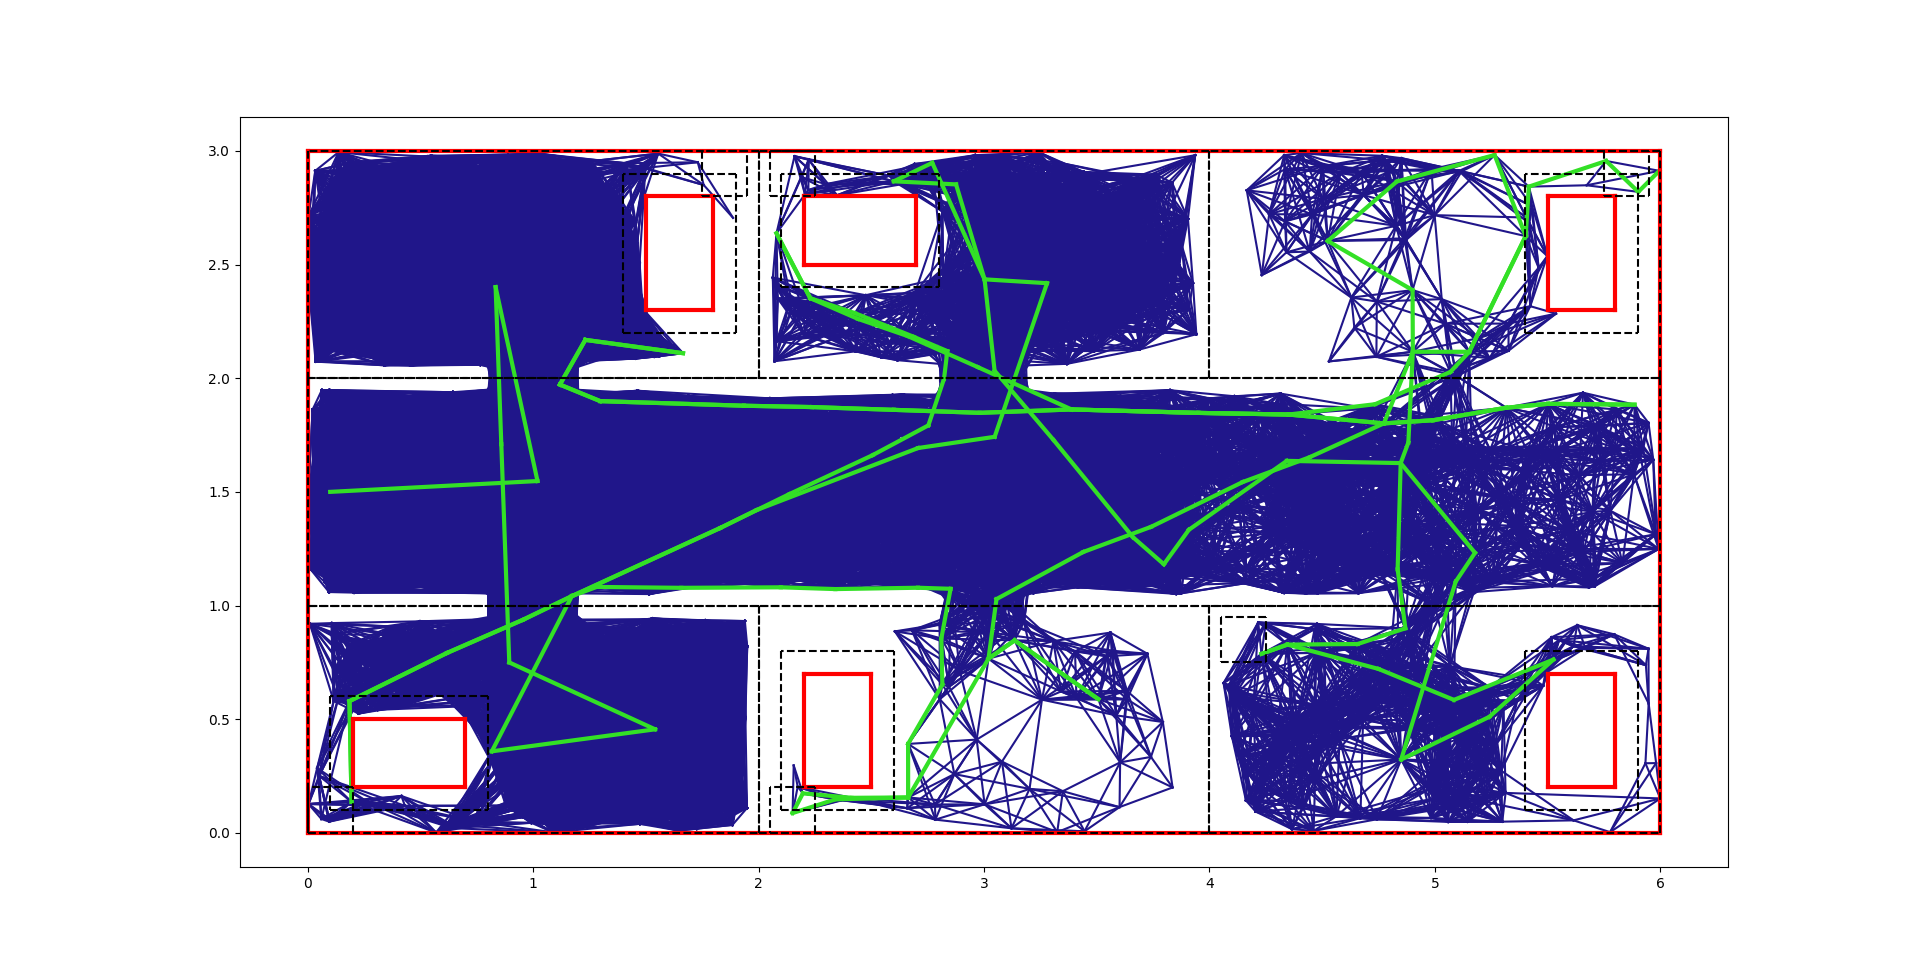
\includegraphics[width=\textwidth]{final.png}
\end{frame}

	
\end{document}